\chapter{State of the Art}
\label{ch:state-of-the-art}

\section{The DNS System: Background}
\label{subsec:2.1}

The \ac{DNS} is the distributed directory that translates human-readable names into machine-readable information — primarily \ac{IP} addresses~\cite{RFC1034,RFC1035}. Its hierarchy mirrors the delegation of administrative authority: the root zone delegates to \ac{TLD}s, which delegate to authoritative name servers for individual domains. Resolution is performed by a recursive resolver acting on behalf of clients — contacting root, \ac{TLD}, and authoritative servers in sequence and caching results for the duration of each record’s \ac{TTL}.

Every \ac{RR} carries a \ac{TTL} governing cache lifetime. \ac{CDN}s use short \ac{TTL}s (60 s or less) for rapid traffic redirection; stable infrastructure records carry \ac{TTL}s of 24 hours or more. For active measurement, two implications follow: (1) querying through a recursive resolver may return stale cached responses; (2) cache state divergence across probes can mimic geographic routing differences. Direct authoritative queries bypass both effects.

\subsection{Resource Record Types Relevant to Measurement Studies}
\label{sec:2.1.1}

\ac{DNS} stores information in typed Resource Records, each serving a distinct purpose \cite{RFC1035}. The record types most relevant to distributed measurement studies are:

\textbf{\ac{A} and \ac{AAAA} records} map a domain name to an \ac{IPv4} or \ac{IPv6} address respectively. A single name may have multiple \ac{A} or \ac{AAAA} records, enabling load distribution through round-robin responses and geographic routing through location-aware \ac{DNS} (different addresses returned depending on the querying resolver's location). This geographic differentiation in \ac{A}/\ac{AAAA} responses is one of the primary phenomena this thesis investigates.

\textbf{\ac{NS} records} designate the authoritative name servers responsible for a \ac{DNS} zone and are essential for identifying the \ac{DNS} infrastructure provider responsible for a domain. Van Rijswijk-Deij~\cite{vanRijswijk2016} include \ac{NS} records in the OpenINTEL standard query set because changes in \ac{NS} delegation reveal infrastructure migrations and provider switches.

\textbf{\ac{MX} records} designate the mail-handling servers for a domain. Van Rijswijk-Deij~\cite{vanRijswijk2016} use longitudinal \ac{MX} analysis as one of two case studies for OpenINTEL, tracking the adoption of cloud email services (Google Workspace, Microsoft Exchange Online, Yahoo Mail) across tens of millions of domains over a ten-month period.

\textbf{\ac{CNAME} records} create an alias pointing from one name to another canonical name. \ac{CDN}s make extensive use of \ac{CNAME} chains: a customer domain (\texttt{www.shop.example}) points to a \ac{CDN}-managed name (\texttt{shop.cdn-provider.net}), allowing the \ac{CDN} to update routing without requiring the customer to change their \ac{DNS} configuration. The same mechanism is used by \ac{DDoS} protection services to divert traffic through their scrubbing infrastructure~\cite{Jonker2016}.


\textbf{DNSKEY, DS, and RRSIG records} are the \ac{DNSSEC} record types carrying public keys, delegation signers, and cryptographic signatures respectively. Van Rijswijk-Deij~\cite{vanRijswijk2016} include all three in the OpenINTEL query set specifically to monitor \ac{DNSSEC} deployment and key management practices at scale. Their longitudinal data revealed systemic key rollover failures invisible to point-in-time measurements.

\textbf{\ac{TXT} records} carry free-text information and are used for \ac{SPF}, \ac{DKIM}, \ac{DMARC} configuration, and domain validation tokens for certificate authorities. Table~\ref{tab:rr_types} summarises the record types relevant to this thesis's measurement campaign.

\begin{table}[H]
\centering
\small
\begin{tabularx}{\linewidth}{p{1.8cm} p{4.1cm} X}
\toprule
\textbf{Type} & \textbf{Content} & \textbf{Relevance for distributed \ac{DNS} measurement} \\
\midrule
\ac{A}     & \ac{IPv4} address(es)                  & Core observable: geographic variation in returned \ac{IP}s indicates \ac{CDN} routing or anycast \\
\ac{AAAA}  & \ac{IPv6} address(es)                  & Parallel to \ac{A}; anycast routing may differ between \ac{IPv4} and \ac{IPv6}~\cite{Bortzmeyer2013} \\
\ac{NS}    & Authoritative name server names   & Identifies \ac{DNS} provider; enables provider migration tracking and centralisation analysis~\cite{Xu2023} \\
\ac{CNAME} & Canonical name alias              & \ac{CDN} delegation chain; resolving the chain reveals the \ac{CDN} operator behind a domain \\
\ac{MX}    & Mail server hostname(s)           & Cloud email adoption tracking~\cite{vanRijswijk2016}; not geographically differentiated \\
\ac{TXT}   & Free-form text                    & \ac{SPF}/\ac{DKIM}/\ac{DMARC} policy; domain ownership verification \\
DNSKEY/DS & \ac{DNSSEC} public key / delegation & \ac{DNSSEC} deployment monitoring; broken chains cause SERVFAIL; 31\% of \ac{DNSSEC} domains have incomplete records~\cite{vanRijswijk2016,Chung2017} \\
\bottomrule
\end{tabularx}
\caption{\ac{DNS} \ac{RR} types relevant to distributed measurement studies. References: \cite{RFC1034,RFC1035}.}
\label{tab:rr_types}
\end{table}

\section{DNS Measurement Paradigms}
\label{sec:2.2}

Measuring \ac{DNS} behaviour at scale can be approached in fundamentally different ways, each with its own trade-offs in terms of coverage, geographic control, and ethical constraints. This section surveys the two main paradigms — passive and active measurement — along with the ethical framework that governs their use, and presents OpenINTEL as the reference large-scale active measurement infrastructure against which this thesis positions itself.

\textbf{Passive \ac{DNS}} captures queries and responses at existing resolvers or \ac{IXPs} without injecting artificial traffic. It reflects real user behaviour and is well suited for security forensics (botnet tracking, phishing detection via commercial services such as Farsight DNSDB). Its fundamental limitation for this thesis is geographic blindness: a passive sensor observes only traffic at its location~\cite{vanRijswijk2016}. It also cannot measure a predefined domain corpus, privacy constraints (GDPR) restrict retention granularity, and the resulting datasets are typically held by commercial operators (Farsight DNSDB, \ac{ISP}s), making them inaccessible for open academic research.

\textbf{Active \ac{DNS} measurement} deliberately sends queries from controlled vantage points, enabling full domain corpus coverage, geographic control, and reproducibility. Van Rijswijk-Deij~\cite{vanRijswijk2016} demonstrate that even at 1.85 billion daily queries for .com alone, well-paced active measurement represents only 0.3–1.6\% of authoritative server traffic — a negligible impact. Van der Toorn~\cite{vanderToorn2018} leverage 180 days of such data to detect snowshoe spam — a technique whereby spammers distribute sending across many domains to evade reputation-based blacklists — with 93\%+ precision and a 100-day lead over blacklists, a result exclusive to the active paradigm. Similarly, Jonker~\cite{Jonker2016} use 1.5 years of daily active measurements to track the adoption of \ac{DDoS} protection services across more than 50\% of the global namespace, revealing a 1.24$\times$ growth in adoption driven by large hosting providers — a trend invisible to any passive or point-in-time approach.

\textbf{Ethical framework}: Kisteleki~\cite{Kisteleki2016} ground RIPE Atlas measurement ethics in the Menlo Report (2012)~\cite{Bailey2012}: researchers bear responsibility for the traffic probe hosts generate. For this thesis, the domain corpus is drawn from publicly accessible Tranco domains; no politically sensitive content is queried; and measurement frequency respects \ac{DNS} \ac{TTL}s.

\textbf{OpenINTEL}~\cite{vanRijswijk2016}, developed at the University of Twente, measures every domain in a \ac{TLD} zone daily from a single vantage point in the Netherlands. It covers over 50\% of the global \ac{DNS} namespace, stores results in Apache Avro/Parquet, and has run continuously since March 2015. Its longitudinal data has supported studies of \ac{DNSSEC} key management failures~\cite{Chung2017}, \ac{DDoS} protection adoption~\cite{Jonker2016}, and cloud email migration~\cite{vanRijswijk2018blog}. Coverage expanded from the initial .com/.net/.org \ac{TLD}s (50\% of the global namespace) to all generic \ac{TLD}s by 2018, and the platform received the Research Data Netherlands Prize in November 2018~\cite{vanRijswijk2018blog}. Its explicit limitation is the single-vantage point architecture: whether a domain returns different \ac{IP} addresses to probes in Japan, Brazil, or South Africa is invisible to OpenINTEL — the primary motivation for the distributed approach of this thesis.


\section{Distributed Measurement: RIPE Atlas}
\label{sec:2.3}

RIPE Atlas is a network of hardware and software probes hosted by volunteers, providing the spatial diversity that OpenINTEL lacks. As of 2024 it comprises approximately 12,900 active probes across 178 countries, generating about 1.3 billion measurement results per day~\cite{Nosyk2025}. \ac{DNS} is a native measurement type: every probe continuously measures all 13 root server addresses, and user-defined campaigns can query any domain, record type, and resolver. Table~\ref{tab:platforms} compares RIPE Atlas with the main alternative platforms.

\begin{table}[H]
\centering
\small
\begin{tabularx}{\linewidth}{p{2.6cm} r p{2.0cm} p{1.8cm} X}
\toprule
\textbf{Platform} & \textbf{Probes} & \textbf{Countries} & \textbf{\ac{DNS} native} & \textbf{Notes} \\
\midrule
RIPE Atlas       & $\approx$12,900 & 178 & Yes & Volunteer hardware probes; credit economy; open academic access~\cite{Nosyk2025} \\
CAIDA Ark        & $\approx$170    & 60+ & No  & Topology-focused; data available on request to academic institutions; limited \ac{DNS} support~\cite{Bajpai2017} \\
SamKnows         & $\approx$70,000 & 50+ & No  & \ac{ISP}-deployed for regulators (FCC, Ofcom); not publicly accessible; broadband QoS focus~\cite{Bajpai2017} \\
PlanetLab        & $\approx$300    & 60+ & No  & Open to academic institutions (slice model); software VMs~\cite{Cicalese2015}; largely inactive since 2020 \\
BISmark          & $\approx$420    & 40+ & No  & Open source but limited access (Georgia Tech); home-network focus; limited geographic diversity~\cite{Bajpai2017} \\
\bottomrule
\end{tabularx}
\caption{Comparison of distributed Internet measurement platforms relevant to \ac{DNS} studies. Probe counts as of 2024 for RIPE Atlas~\cite{Nosyk2025} and approximately 2017 for others~\cite{Bajpai2017}. RIPE Atlas is the only platform with native \ac{DNS} measurement support and open academic access at global scale.}
\label{tab:platforms}
\end{table}

\textbf{Probe selection}: Bajpai~\cite{Bajpai2017} distinguish system tags (automatically derived from RIPE Atlas built-in measurements every four hours, reliable) from user tags (manually set by probe hosts; only 2.8\% ever update them, making them frequently stale). The recommended selection protocol is: filter by system tags (system-ipv4-works, system-resolves-a-correctly), then stratify geographically to compensate for the 91\% Europe/North America concentration. Holterbach~\cite{Holterbach2015} further document measurement interference: concurrent campaigns on the same probes introduce timing errors of 1–7 ms and temporal desynchronisation of up to one hour. Scheduling at off-peak times and using repeated measurements mitigate both effects.

\textbf{Geographic bias}: Germany and the USA together account for 28\% of all probes; Africa, Latin America, and Southeast Asia are substantially under-represented relative to Internet user populations~\cite{Nosyk2025}. Figure~\ref{fig:ripe_atlas_distribution} maps this distribution. Geographic stratification during probe selection is therefore mandatory for any study of global \ac{DNS} variation.

\begin{figure}[tp]
  \centering
  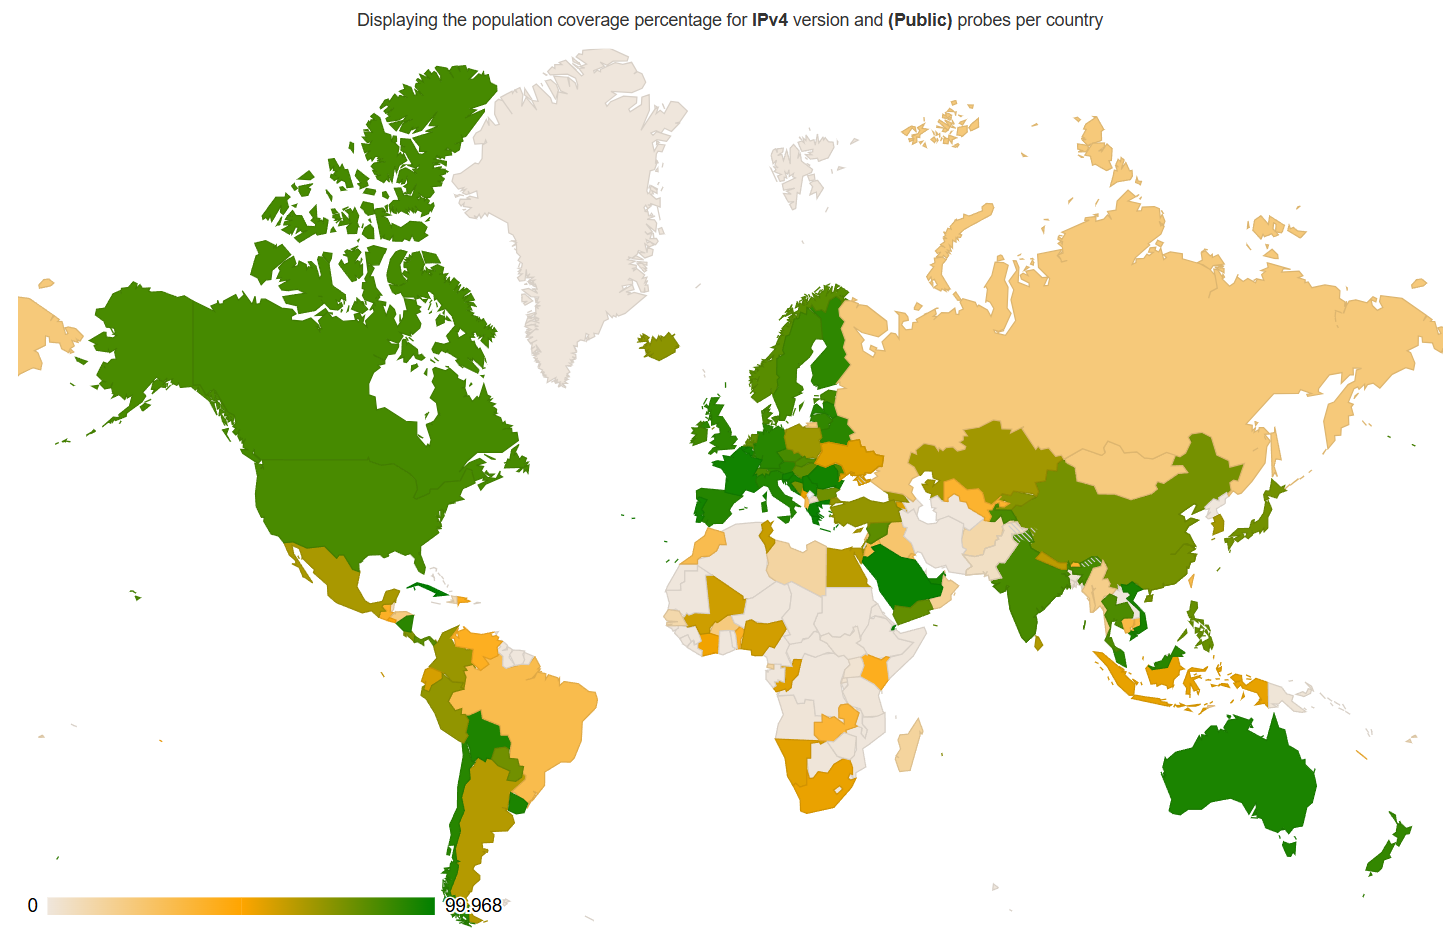
\includegraphics[width=0.90\linewidth]{figures/fig3b_ripe_atlas_distribution.png}
  \caption{Number of connected RIPE Atlas probes and anchors per country in March 30, 2026. Source: RIPE Atlas}
  \label{fig:ripe_atlas_distribution}
\end{figure}

\textbf{Measurement validity}: Jones~\cite{Jones2016} detect in-path transparent \ac{DNS} proxies in ten \ac{ISP}s: a Kenyan \ac{ISP}’s proxy answers root \ac{DNS} queries 23× faster than the actual B-root \ac{RTT} (14 ms vs. 318 ms). Nosyk~\cite{Nosyk2025} find that 69\% of Chinese probes fail to resolve Meta domains — geographic filtering, not measurement failure. These findings require two data quality steps: \ac{RTT} sanity checks to identify proxied probes, and cross-domain cross-temporal analysis to distinguish censorship from hardware failure. Boswell and Perkins~\cite{Boswell2024} further show that 3,092 internal domain names are actively used by RIPE Atlas probes, with 34.5\% at risk of name collision if their \ac{TLD} is globally delegated — a finding that underlines the need to validate probe resolution behaviour before including probes in \ac{DNS} corpus measurements.

\section{Anycast Routing in DNS}
\label{sec:2.4}

\ac{IP} anycast is the dominant routing architecture for \ac{DNS} root servers, \ac{TLD} servers, and major public resolvers (Google 8.8.8.8, Cloudflare 1.1.1.1). Probes at different geographic locations may contact physically different servers behind the same anycast \ac{IP}; the responses may differ in latency and, when servers are misconfigured or \ac{BGP} routing is suboptimal, in content. Three aspects of anycast are particularly relevant to distributed \ac{DNS} measurement: how to identify which physical instance answered a query, how \ac{BGP} topology shapes the geographic distribution of queries across instances, and how \ac{IPv4} and \ac{IPv6} routing can diverge for the same anycast address.

\textbf{Instance identification}: A prerequisite for anycast measurement is knowing which physical server instance actually answered the query. Two complementary techniques address this. The \ac{NSID} option (~\cite{RFC5001}) causes the responding server to embed an identifier in its response (e.g., \texttt{dns.th2.nic.fr} for the Paris instance of \texttt{d.nic.fr}). The id.server CHAOS query (~\cite{RFC4892}) returns an IATA-code identifier (e.g., ams, fra); because CHAOS class records are not cached, each query reaches the live \ac{BGP}-routed instance~\cite{Finnegan2018}. Without one of these mechanisms, two probes receiving identical \ac{A} records cannot be distinguished from a routing standpoint.

\textbf{\ac{BGP} attraction basins}: Once instance identity can be established, the question becomes: what governs which probes reach which instance? Bortzmeyer~\cite{Bortzmeyer2013} demonstrates for \texttt{d.nic.fr} that anycast routing is governed by \ac{BGP} peering topology rather than physical distance. For instance, while one might expect North American queries to be routed to the geographically closest available node, 55\% are sent to Paris and 33\% to Frankfurt — showing that network closeness in \ac{BGP} does not align with mileage. Finnegan~\cite{Finnegan2018} confirms this pattern for UncensoredDNS with 500 Atlas probes. This has a direct consequence for this thesis: geographic probe diversity does not guarantee instance diversity, and response differences between probes may reflect \ac{BGP} topology rather than intentional geographic routing.

\textbf{\ac{IPv4}/\ac{IPv6} divergence}: A further complication arises because \ac{IPv4} and \ac{IPv6} \ac{BGP} tables are maintained independently, potentially routing the same anycast prefix to different physical instances. Bortzmeyer~\cite{Bortzmeyer2013} documents a reversal for \texttt{d.nic.fr}: Frankfurt is the dominant \ac{IPv6} instance (36\% of global queries) but subordinate in \ac{IPv4} (17\%). Dual-stack measurements must therefore be run and analysed separately to avoid conflating two distinct routing dimensions. Koch~\cite{Koch2021} further show that anycast inflation (routing to a suboptimal replica) affects over 95\% of users for at least one \ac{DNS} root letter, though its practical impact is negligible for root \ac{DNS} because root records are cached for six days.

\section{CDN Routing and EDNS Client Subnet}
\label{sec:2.5}

\ac{CDN}s use \ac{DNS} as the primary mechanism to direct each client to a geographically appropriate server replica. The \ac{CDN}’s authoritative server returns a different \ac{A}/\ac{AAAA} record depending on the inferred location of the querying resolver. Li~\cite{Li2025}, studying Twitch, find continent-level \ac{DNS} routing granularity: distinct \ac{IP} groups are returned to probes in Europe, North America, and Asia-Pacific, creating sharp geographic boundaries detectable by distributed active measurement.

\textbf{The remote \ac{DNS} problem}: \ac{DNS}-based \ac{CDN} routing assumes the recursive resolver is near its clients. When clients use a public resolver (Google 8.8.8.8, Cloudflare 1.1.1.1), the \ac{CDN} sees the resolver’s location rather than the client’s. Hours~\cite{Hours2016} quantify this causally using passive \ac{ISP} traces: clients using Google \ac{DNS} receive Akamai servers 20 ms farther in \ac{RTT} on average, with a secondary 14\% throughput reduction from smaller server congestion windows. Wang~\cite{Wang2018} find public \ac{DNS} adoption growing at 27\% per year and mismatches reaching 113\% in server distance — more than twice the optimal assignment.

\textbf{\ac{ECS}}~\cite{RFC7871} addresses this by embedding the client’s /24 \ac{IP} prefix in the query forwarded to the authoritative server. The \ac{CDN} uses this prefix (not the resolver \ac{IP}) for server selection. \ac{ECS} introduces a privacy trade-off: the client’s network location becomes visible to the authoritative server and any on-path observer. RFC 7871 recommends disabling \ac{ECS} by default. In practice, Bortzmeyer~\cite{Bortzmeyer_tutorial} finds that most RIPE Atlas probes use resolvers that do not forward \ac{ECS}, so responses are typically resolver-\ac{IP}-determined. To opt out of \ac{ECS} explicitly, SOURCE PREFIX-LENGTH = 0 can be set in the query. Figure~\ref{fig:ecs_schema} illustrates all three \ac{ECS} scenarios.

\begin{figure}[tp]
  \centering
  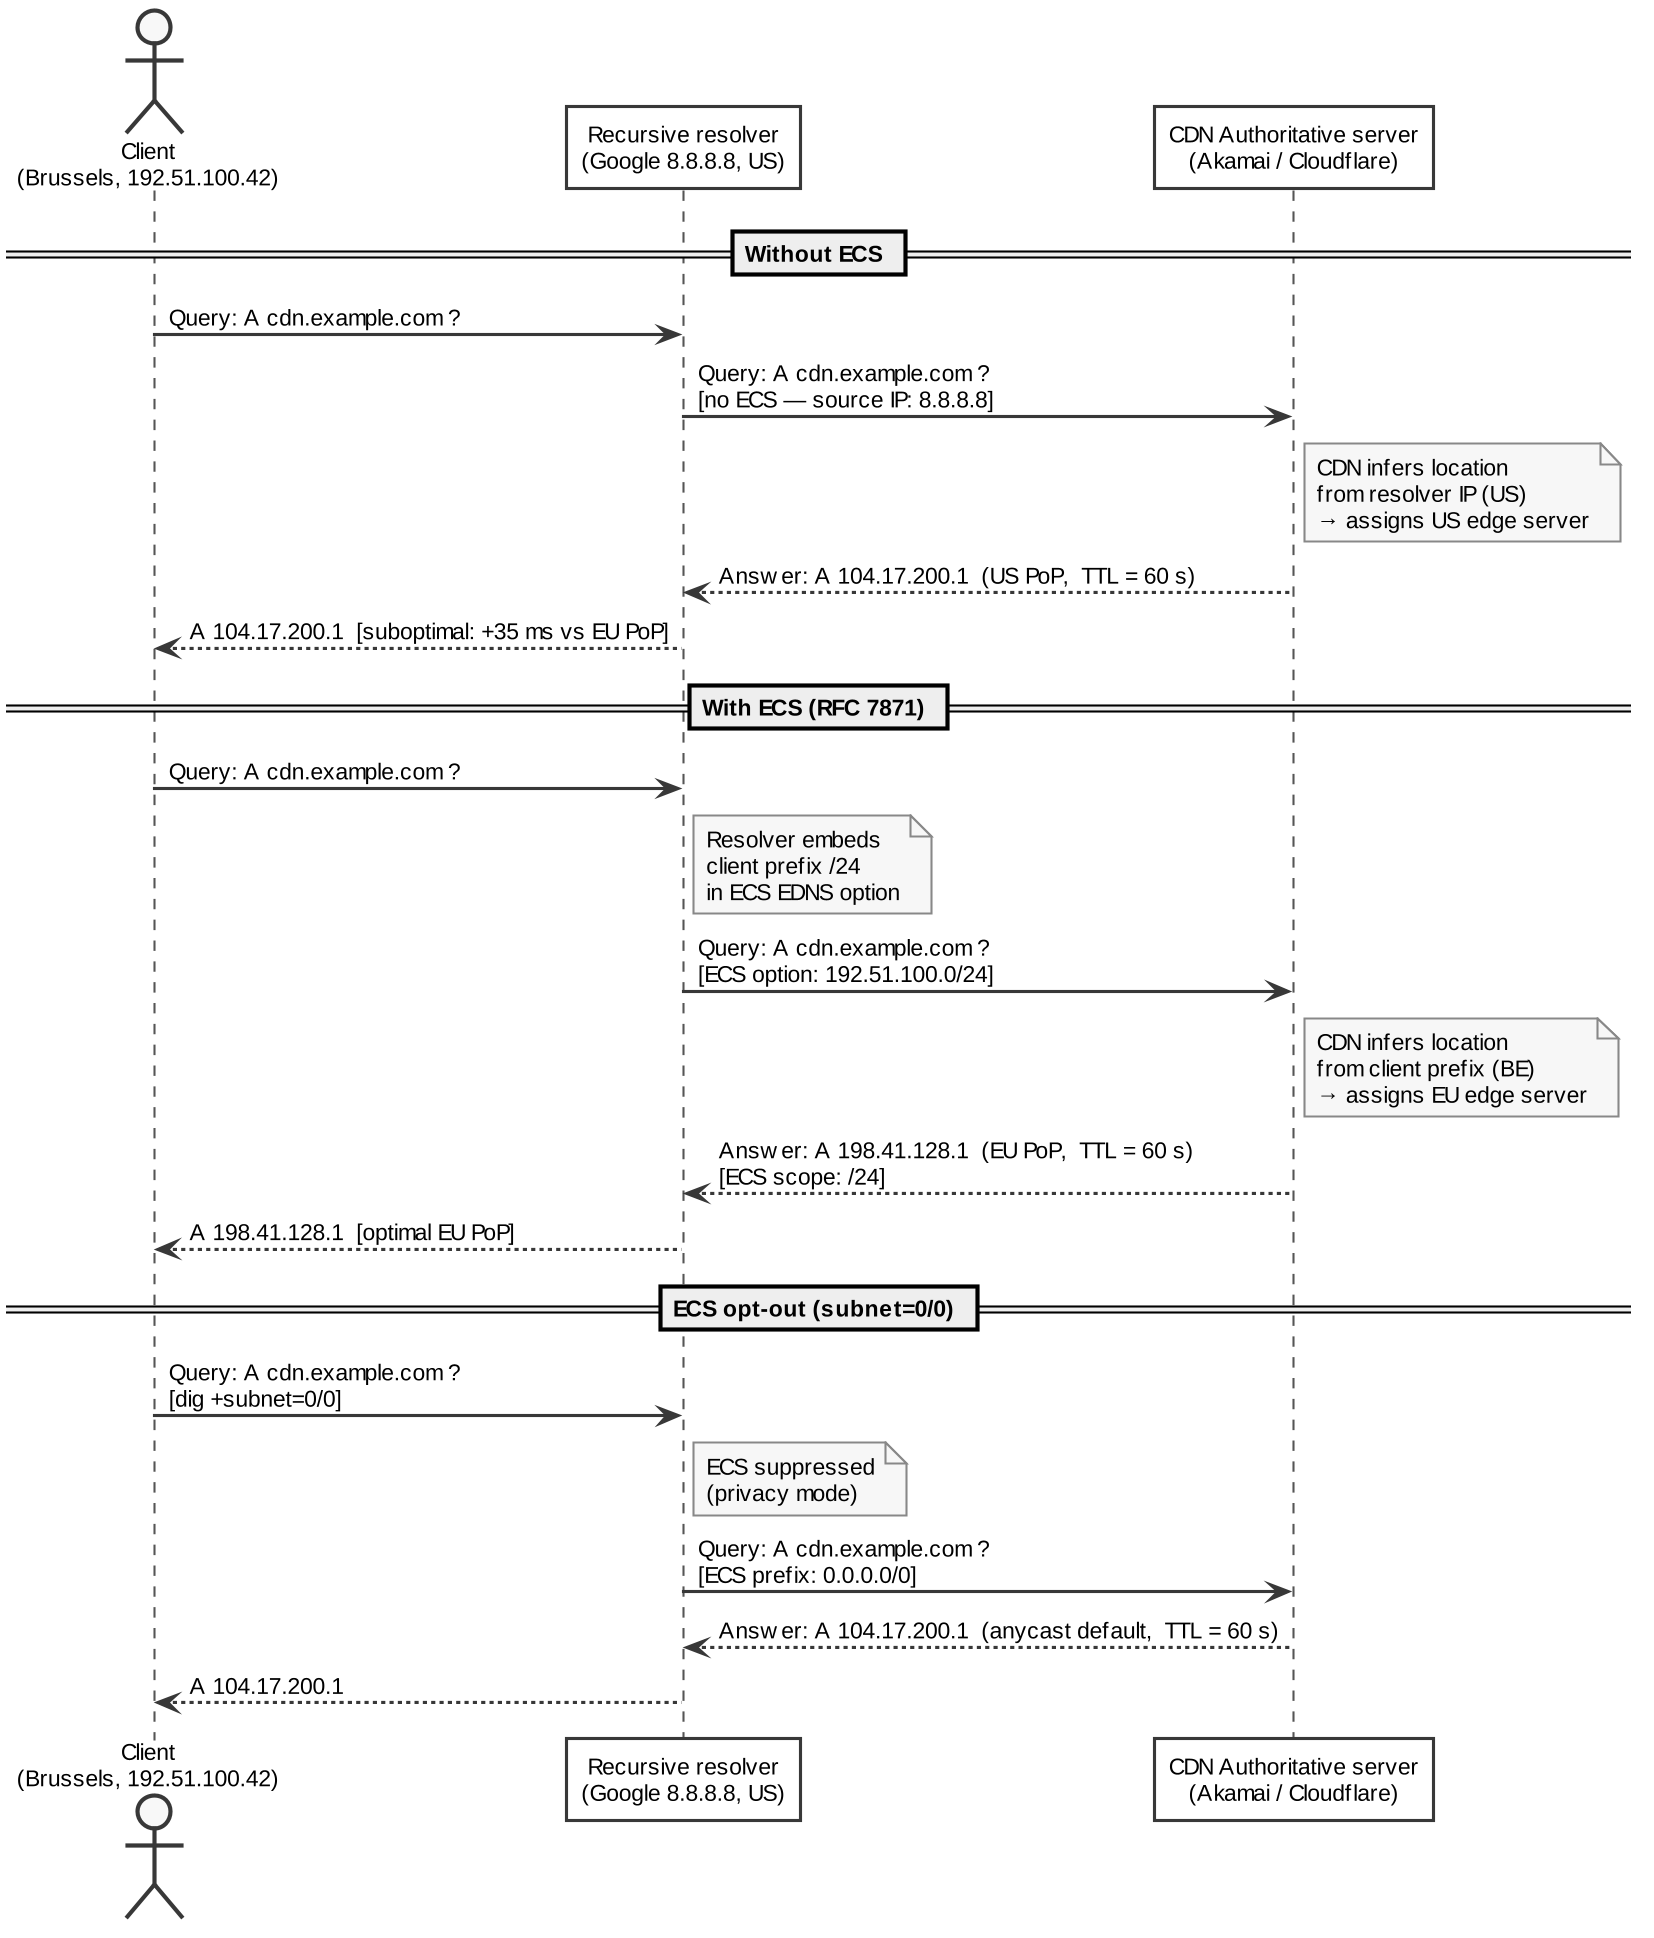
\includegraphics[width=0.90\linewidth]{figures/fig4_ecs_schema.png}
  \caption{Effect of \ac{ECS}~\cite{RFC7871} on \ac{CDN} geographic routing. \textit{Without \ac{ECS}}, the \ac{CDN} authoritative server infers client location from the recursive resolver's \ac{IP} (8.8.8.8, US), assigning a suboptimal US edge server to a Belgian client. \textit{With \ac{ECS}}, the resolver embeds the client's /24 prefix; the \ac{CDN} selects the geographically appropriate EU \ac{PoP}. \textit{\ac{ECS} opt-out} (\texttt{subnet=0/0}) suppresses the prefix entirely, reverting to resolver-\ac{IP}-based routing.}
  \label{fig:ecs_schema}
\end{figure}

\textbf{\ac{DNS} infrastructure centralisation}: Xu~\cite{Xu2023} show that over 90\% of forwarding resolvers are backed by fewer than 5\% of indirect recursive resolvers, and that just 10 \ac{DNS} providers serve 48.5\% of all g\ac{TLD} domain names. This centralisation creates a methodological choice between two complementary approaches, each with distinct trade-offs.

\textit{Using the probe's default resolver} reflects the experience of real end-users: queries traverse the full recursive resolution chain, including the \ac{ISP} resolver's cache and any \ac{ECS} forwarding behaviour. This approach is appropriate for studying \ac{DNS} as users actually encounter it. Its limitation is that geographic diversity of probes may be partially illusory: two probes from different continents may share the same upstream recursive resolver, making their responses indistinguishable regardless of probe location.

\textit{Querying authoritative servers directly} — by targeting the authoritative name server's \ac{IP} and clearing the \ac{RD} bit — bypasses recursive resolvers entirely. Each probe's query reaches the authoritative server from its own \ac{IP} address, isolating the geographic routing signal produced by the authoritative infrastructure. The limitation is that results do not reflect what users actually receive through their resolver chain. RIPE Atlas natively supports both modes.

This thesis uses direct authoritative queries for Q1–Q3, where the goal is to characterise how the authoritative infrastructure responds to different geographic origins, and the probe's default resolver for Q4, where the goal is precisely to compare resolver-induced differences in returned responses.

\section{Domain Ranking Lists}
\label{sec:2.6}

Studies of \ac{DNS} behaviour at scale require a reproducible domain corpus. Le Pochat~\cite{LePochat2019} evaluate four freely available ranking lists — Alexa, Cisco Umbrella, Majestic, and Quantcast — and find they agree on only 70,000 of a combined 2.82 million unique domains (24–33\% rank-biased overlap). Alexa’s 2018 methodology change caused 50\% daily list turnover, making longitudinal studies unreliable; Amazon subsequently shut down the Alexa ranking service entirely on 1 May 2022, making it unavailable for any ongoing research. Cisco Umbrella contains 51\% non-web entries (EC2 hostnames, typos). Majestic contains 2,162 documented malicious domains. All four lists are trivially manipulable: a single \ac{HTTP} request from an Alexa browser extension user can lift a domain to rank 28,798. Table~\ref{tab:ranking_lists} compares the main properties.

\begin{table}[tp]
\centering
\small
\begin{tabularx}{\linewidth}{p{2.2cm} X X X X}
\toprule
\textbf{Property} & \textbf{Alexa} \newline \textit{(discontinued 2022)} & \textbf{Cisco Umbrella} & \textbf{Majestic} & \textbf{Tranco} \\
\midrule
Data source  & Browser extension & \ac{DNS} queries to OpenDNS & Web crawl backlinks & Multi-source aggregation \\
Daily change rate & $\approx$50\,\% (post-2018) & $\approx$10\,\% & $\approx$1\,\% & $\approx$0.6\,\% \\
Manipulation effort & 1 \ac{HTTP} request & 1 \ac{DNS} query injection & Few backlinks & 4$\times$ vs single-source \\
Non-domain entries & Low & $\approx$51\,\% & Low & Filtered \\
Malicious domains & Some & Some & 2\,162 documented & Filtered \\
Reproducibility   & Daily overwrite & Daily overwrite & Daily overwrite & Stable permalink \\
\bottomrule
\end{tabularx}
\caption{Comparison of domain ranking lists. Tranco is the only list designed for research reproducibility and manipulation resistance~\cite{LePochat2019}.}
\label{tab:ranking_lists}
\end{table}

\textbf{Tranco} \cite{LePochat2019} aggregates multiple lists over a 30-day rolling window using the Borda count, producing a stable corpus (0.6\% daily change), resistant to manipulation (requires quadrupled effort across multiple lists), and reproducible via stable archived permalinks. For this thesis, Tranco’s stability guarantees that the same domain set is measured across 60 daily campaigns, enabling meaningful temporal comparison.

\section{Synthesis and Research Positioning}
\label{sec:2.7}

The preceding review reveals a clear gap at the intersection of OpenINTEL’s temporal depth and RIPE Atlas’s spatial diversity. OpenINTEL provides daily, \ac{TLD}-wide \ac{DNS} measurement since 2015 but from a single Dutch vantage point: geographic variation is invisible. Existing RIPE Atlas \ac{DNS} studies are predominantly single-campaign, domain-limited case studies (a few hundred domains, one time point): Bortzmeyer~\cite{Bortzmeyer2013} studies a single anycast server; Finnegan~\cite{Finnegan2018} measures one resolver with 500 probes at a single instant; Hours~\cite{Hours2016} targets a handful of \ac{CDN} providers in one campaign; Koch~\cite{Koch2021} analyses root server anycast at one point in time. No study has systematically characterised what fraction of popular domains return geographically differentiated \ac{DNS} responses, which mechanisms drive that differentiation, or how differentiation evolves over months. Table~\ref{tab:gap_analysis} formalises this positioning.

\begin{table}[tp]
\centering
\small
\begin{tabularx}{\linewidth}{p{2.8cm} p{3.5cm} p{3.8cm} X}
\toprule
\textbf{Dimension} & \textbf{OpenINTEL-based studies}~\cite{vanRijswijk2016} & \textbf{Existing RIPE Atlas studies}~\cite{Bortzmeyer2013,Finnegan2018,Hours2016,Koch2021} & \textbf{This thesis} \\
\midrule
Domain coverage  & Full \ac{TLD} zone files & Experimenter-defined (per study) & Tranco Top-250 (stable, reproducible) \\
Geographic vantage    & Single point (Netherlands) & $\approx$12\,900 probes, 178 countries & Multi-continent stratification \\
Temporal depth & Daily since March 2015 & Single campaigns & 60-day repeated campaigns \\
Anycast tracking       & Not applicable & Case studies (d.nic.fr, UncensoredDNS) & Systematic across corpus \\
Resolver control   & Fixed central resolver & Local probe resolver (default) & Direct authoritative query \\
\bottomrule
\end{tabularx}
\caption{Positioning of this thesis relative to existing \ac{DNS} measurement infrastructure across five dimensions.
All three columns represent measurement studies; Each row identifies a gap that this work explicitly addresses.}
\label{tab:gap_analysis}
\end{table}

Three specific gaps drive the contribution:

\textbf{Gap 1 — No population-scale geographic \ac{DNS} characterisation}: Individual anycast case studies (\cite{Bortzmeyer2013}; \cite{Finnegan2018}) and \ac{CDN} routing studies (\cite{Hours2016,Li2025}) target one service or domain at a time. No study has measured what fraction of the popular-domain corpus returns geographically differentiated responses, nor which mechanisms dominate at scale.

\textbf{Gap 2 — Resolver centralization undermines vantage-point diversity}: Using local probe resolvers creates apparent geographic diversity that disappears at the resolution layer (90\% of forwarding resolvers → 5\% of recursive resolvers, \cite{Xu2023}). Direct authoritative querying is the required mitigation, but none of the cited case studies document it as an explicit design choice.

\textbf{Gap 3 — Single-campaign studies miss temporal dynamics}: Koch~\cite{Koch2021} and Bortzmeyer ~\cite{Bortzmeyer2013} acknowledge that \ac{BGP} routing and \ac{CDN} anycast catchments change over time as operators add \ac{PoPs} or renegotiate peering. A 60-day longitudinal campaign is necessary to characterise the stability of geographic \ac{DNS} response differentiation.

This thesis addresses all three gaps by deploying a measurement system that queries the Tranco Top-250 directly at authoritative servers from $\approx$200 geographically stratified RIPE Atlas probes, repeated daily over 60 days, with \ac{NSID}-based anycast instance tracking and results archived in Parquet following \ac{FAIR} data principles.